%****************************************************
%	CHAPTER 1 - INTRODUCTION
%****************************************************
\chapter{Introduction}
\label{ch:introduction}
%====================================================
\section{Background}
\label{sec:ch1.background}
%====================================================
\subsection{Radar and Applications}
\label{subsec:ch1.section1.radarapplications}
%----------------------------------------------------
The field of radar gained popularity decades ago. It's uses back then were limited to target detection mostly, and the technology has since expanded to achieve much more sophisticated functionality.
As per its origins, radar stands for Radia Detection And Ranging. Radar systems can be described as systems that use electromagnetic technology in the high frequency range to detect, classify and track targets.
Such targets may include aircraft, ships, vehicles, weather balloons, and even incoming weather formations such as precipitation and storms. The technology has adapted to a wide range of applications, including air traffic control, weather monitoring, military defense, and autonomous vehicles.
What was once a military technology designed for defense purposes is now an extremely useful tool, capable of helping many of our modern day industries.

That said, the focus of this project's application is the tracking of moving airborn vehicles. This project hopes to contribute to the tracking of a weather balloon system being developed at UCT; however, this project will focus on detecting aircraft around Cape Town International airport for ease of testing.

%====================================================
\subsection{Types of Radar}
\label{subsec:ch1.section1.typesofradar}
%----------------------------------------------------
There are various types and subtypes of radar systems, each with their own applications. 
Active radar systems transmit their own signals and measure reflections off of targets to detect. Passive radar on the other hand, relies on external sources of transmission -- such as broadcast radio stations -- to transmit electromagnetic signals, which reflect off moving targets and -- once captured and analysed -- can provide detection of such targets. While passive radar systems are more energy efficient due to the lack of transmitting sigbals, they are reliant on external, third party transmissions which may be of poor quality, affecting the subsequent accuracy of detections.
To mitigate false detections and seperate the direct signal from its echoes, a range of complex mathematical algorithms and transformations are applied to the received signals. These algorithms must be chosen with care to maximise detection robustness and reliability, whilst allowing the system to keep up real-time processing.

% \begin{figure}[H]
%     \centering
%     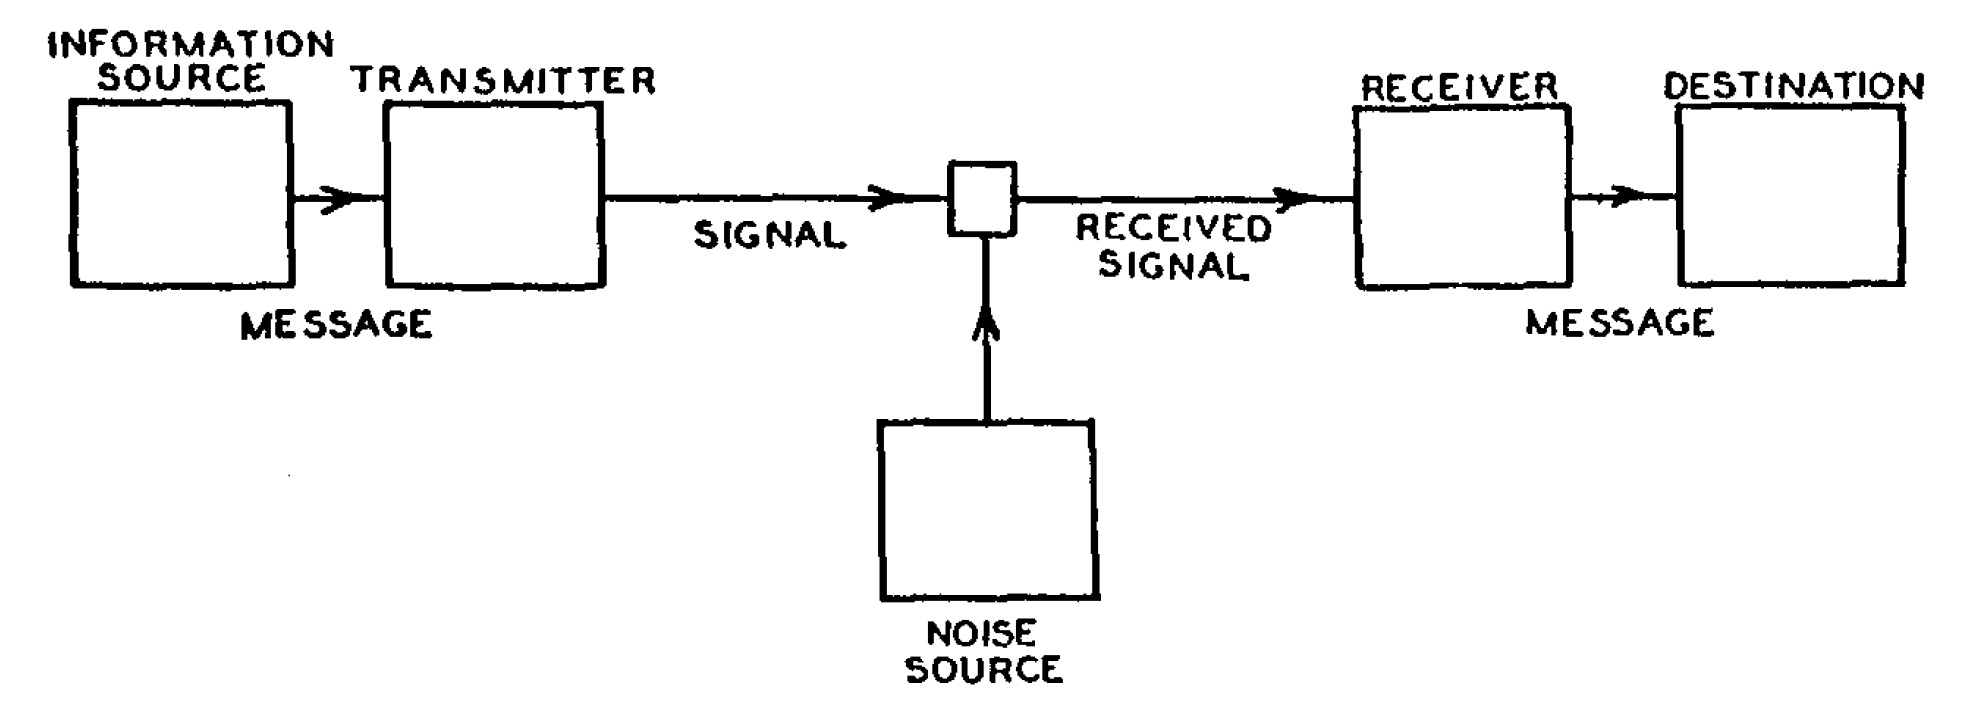
\includegraphics[width=0.8\textwidth]{figs/ch1/shannon.jpg}
% \caption[A simplified block diagram of a general communication system.]{\textbf{A simplified block diagram of a general communication system.} A communication system can be abstracted as follows: an \textit{information source} produces a message to be sent through a \textit{transmitter} which converts it to a signal which can be sent via a communication \textit{channel}. The received signal is noisy and is converted back to the message by the \textit{receiver} which is then delivered to the \textit{destination}. Taken from \cite{shannon1948}.}
%     \label{fig:my_label}
% \end{figure}
%----------------------------------------------------
\pagebreak
%----------------------------------------------------
% \begin{table}[H]
%     \centering
%     \caption[Table title]{\textbf{Table title.} Extended description of tables contents.}
%     \begin{tabularx}{\textwidth}{>{\raggedright\arraybackslash}m{8cm}>{\raggedright\arraybackslash}X>{\raggedright\arraybackslash}X}
%     \toprule[2.25pt]
%     \multirow{3}{*}{\textbf{Heading 1}}        &  \multicolumn{2}{c}{\textbf{Heading 2}}   \\
%     \cmidrule[0.5pt](lr){2-3}
%     &  \multicolumn{1}{c}{\textit{\small Subheading 1}} & \multicolumn{1}{c}{\small \textit{Subheading 2}}\\
%     &  \multicolumn{1}{c}{\small [units]} & \multicolumn{1}{c}{\small [units]}\\
%     \midrule[1pt]
%          &  &\\
%          &  &\\
%          &  &\\
%     \bottomrule[2.25pt]
%  \end{tabularx}

%     \label{table:my_label}
% \end{table}


%====================================================
\section{Problem statement}
\label{sec:ch1.problemstatement}
%====================================================
% Equations are numbered and include the chapter number. As they are considered part of the text, they include punctuation, and each parameter must be described in the text below. Ensure that the units are stated and where possible use SI units. For example, the Maxwell equations are expressed as:
% \begin{align}
% \nabla \cdot \bm{E} &= \frac{\rho}{\epsilon_0}, \\
% \nabla \cdot \bm{B} &= 0, \\
% \nabla \times \bm{E} &= -\frac{\partial \bm{B}}{\partial t}, \\
% \nabla \times \bm{B} &= \mu_0 \bm{J} + \mu_0 \epsilon_0 \frac{\partial \bm{E}}{\partial t},
% \end{align}

% where $\bm{B}$ is the magnetic flux density in T, $\bm{J}$ is the total current density in A/m$^2$, $\bm{E}$ is the electric field in V/m, $\mu_0$ is the permeability of free space (4\(\pi \times 10^{-7}\) H/m), and $\epsilon_0$ is the permittivity of free space (8.85 \(\times 10^{-12}\) C$^2$/N·m$^2$).


%====================================================
\section{Project objectives}
\label{sec:ch1.projectobjectives}
%====================================================
% The \gls{gps} is used for positioning. The \gls{miz} is of particular interest in the \gls{so}.
%====================================================
\section{Scope, limitations and assumptions}
\label{sec:ch1.scope}
%====================================================
%====================================================
\section{Plan of development}
\label{sec:ch1.planofdevelopment}
\pagebreak
%====================================================
%----------------------------------------------------
%****************************************************
% END
%****************************************************
